\documentclass[dvipsnames,beamer]{standalone}
\usepackage[T1]{fontenc}
\usepackage[utf8]{inputenc}

\usepackage{textcomp}
\usepackage{lmodern}


%\usepackage[
%	backend=biber,
%	maxbibnames=99,
%	style=alphabetic,
%	backref=false,
%]{biblatex}
%\bibliography{../cryptobib/abbrev3,../cryptobib/crypto,../standards,../customrefs}

\usepackage{tikz}
\usetikzlibrary{positioning,decorations.pathreplacing,fit}
\usetikzlibrary{decorations.markings,arrows.meta,shapes.arrows,arrows}
\usetikzlibrary{calc}

\definecolor{mygreen}{RGB}{0,128,80}
\colorlet{darkgreen}{mygreen!90!black}


\begin{document}

%\small

\begin{standaloneframe}


\resizebox{\textwidth}{!}{

\begin{tikzpicture}[
	>=triangle 60,
	arrow double line/.style={
		double distance = 20pt,
   		shorten <= 11.5, 	
   		shorten >= 16.1,
   		very thick,
	    postaction = {
    		draw = white,
	 	    line width = 20pt,
	 	    shorten <=-.1pt,
	 	    shorten >=-.1pt,	
	    },
	    postaction = {
	    	decorate, 
	    	decoration = {
	    		markings, 
	    		mark=at position 0 with {
	    			\arrow[xshift=26.6pt]{Straight Barb[reversed,length=-1pt 0.7]}
	    		},
	    		mark = at position 1 with {
   	    			\arrow[xshift=10.6pt]{Straight Barb[length=-1pt 0.7]}
   	    		}
	    	}
	    }
	},
	mysingle/.style = {
		double distance = 22,
		shorten <= 10.5, 	
		shorten >= 14,
		very thick,
		postaction = {
	 		draw = white,
			line width = 22pt,
			shorten <=8pt,
			shorten >=-.5pt,	
		},
		postaction = {
			decorate, 
			decoration = {
				markings, 
				mark = at position 1 with {
					\arrow [xshift=15]{Straight Barb[length=15]}
				}
			}
		},	
	},
	mybrace/.style= {
		decorate, decoration={brace,amplitude=5pt,raise=5pt}, thick
	},
	comment box/.style = {
		draw,inner sep = 6pt,fill=gray!25,thick,rounded corners=3pt,text=black,font=\large
	},
	every node/.style={
		font=\bfseries
	},	
	]

	

		
	\node[] (client) {Client};
	\node[right = 4.3 of client] (AP) {Access point};
	\node[right = 4.0 of  AP] (AS) {Server};
	\def\InterMsgSpaceVertical{1.2}
	

	\node[inner sep=0pt, xshift=0cm,yshift=0.8cm] (laptop_icon) at (client) {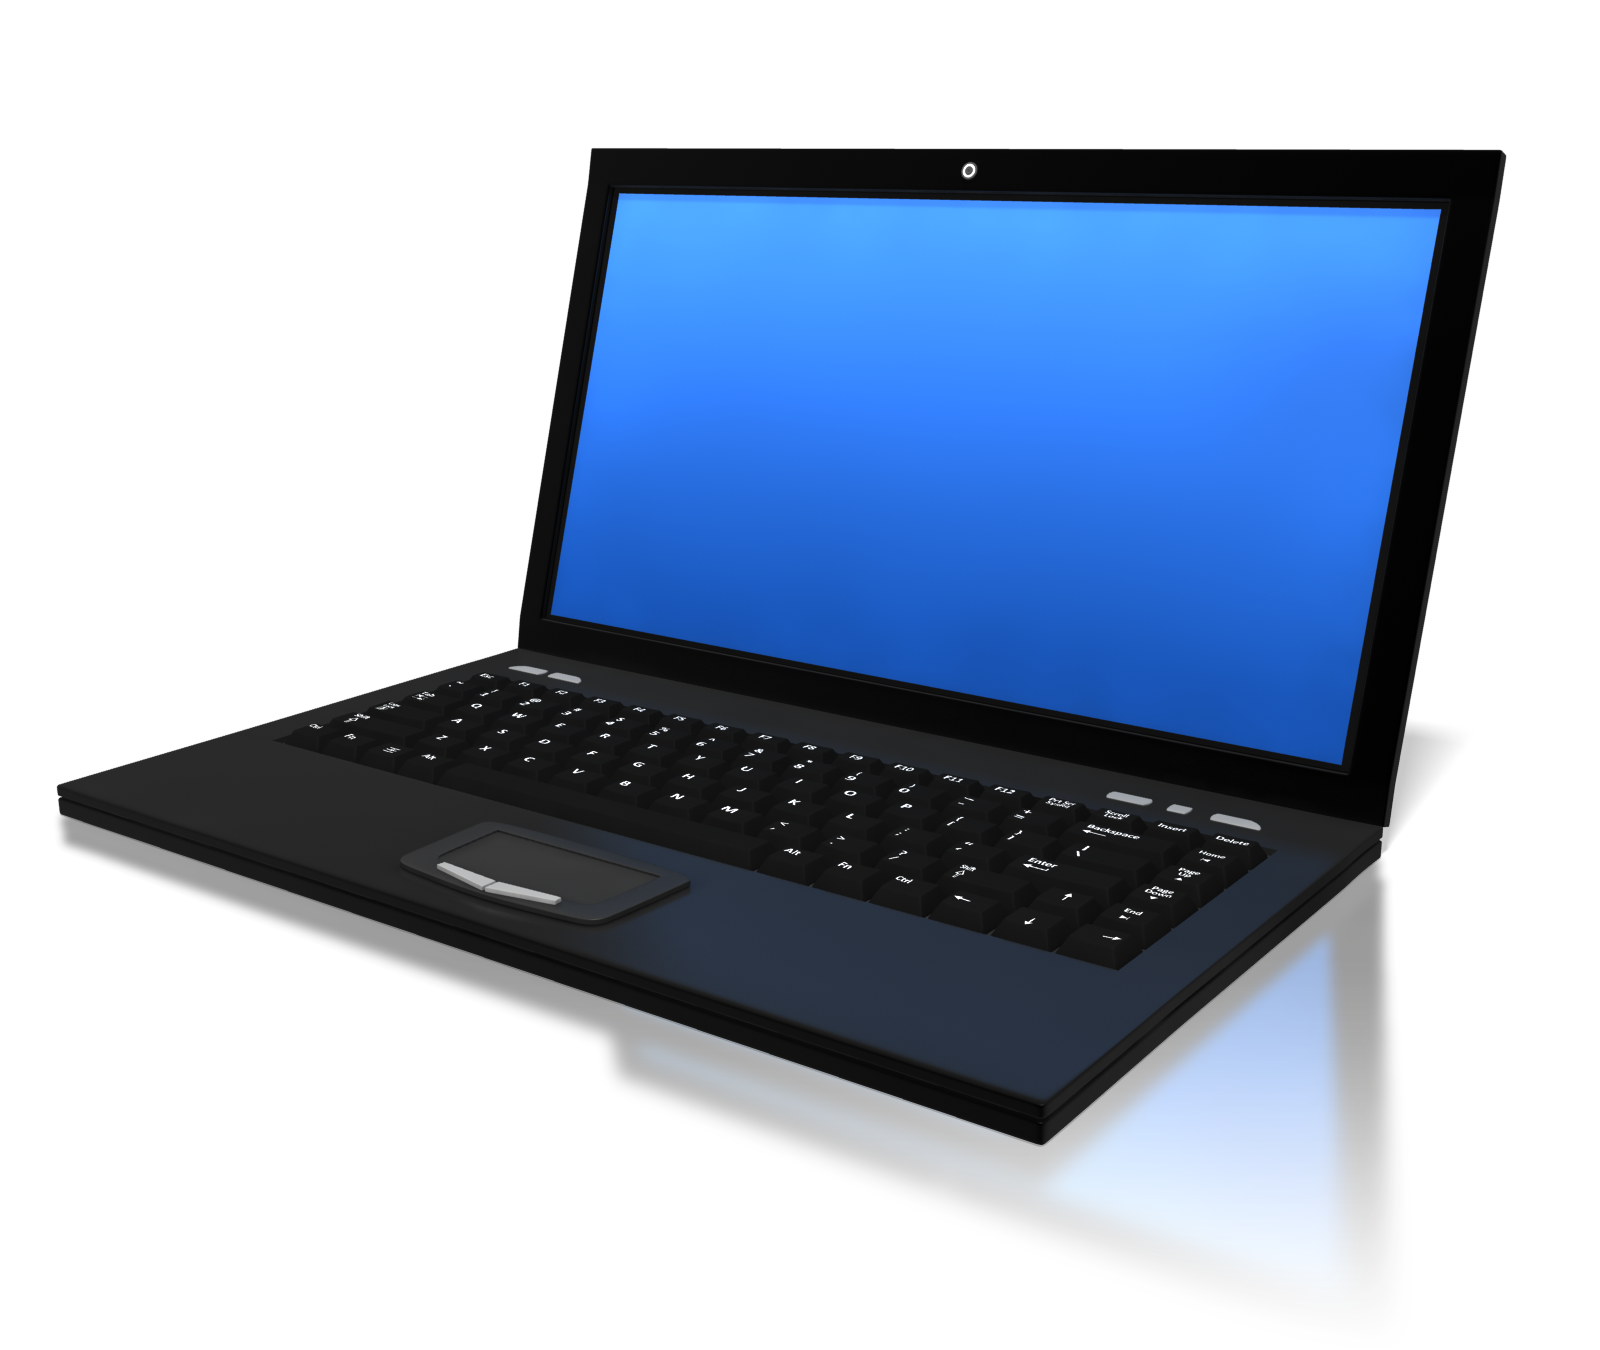
\includegraphics[width=.15\textwidth]{laptop}};
	
	\node[inner sep=0pt, xshift=-0.0cm,yshift=1.1cm] (AP_icon) at (AP) {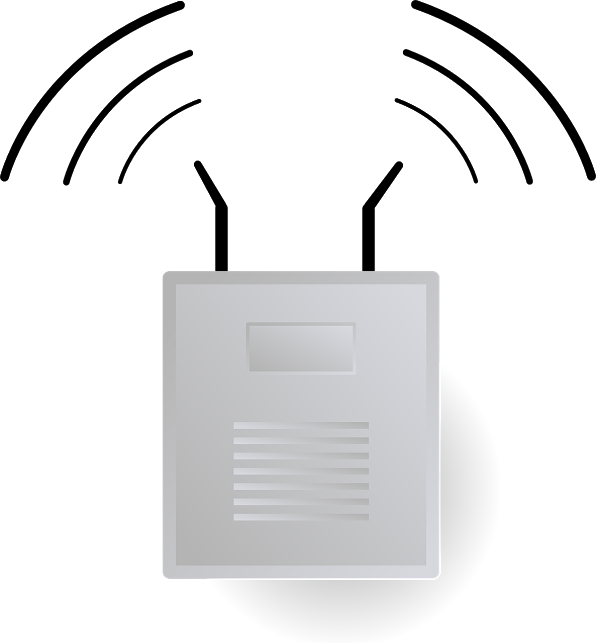
\includegraphics[width=.13\textwidth]{AP}};


	\node[above = -0.2 of AS] () {
\includegraphics[width=.1\textwidth]{server}};

	
	\foreach \i in {1,...,8} {
		\coordinate[below = \InterMsgSpaceVertical * \i of client] (c\i) {};
		\coordinate[below = \InterMsgSpaceVertical * \i of AP] (ap\i) {};
		\coordinate[below = \InterMsgSpaceVertical * \i of AS] (as\i) {};
	}
	
	
	
	\draw[arrow double line,red] (c1) -- node (EAP) {EAP-TLS} (as1);


	\draw[arrow double line,blue] (ap2) -- node[xshift=-2] (AAA) {\temporal<7>{Key Transport}{RADIUS}{RADIUS-over-TLS}} (as2);

	\draw[arrow double line,darkgreen] (c3) -- node[xshift=-2] (4whs) {\alt<2->{4-Way Handshake}{IEEE 802.11}} (ap3);


	\visible<1>{
		\draw[mybrace, decoration={mirror}, left] ([xshift=-0.8cm,yshift=15]c1) -- node[left=0.4,align=center] {WPA2\\Enterprise} ([xshift=-0.8cm,yshift=-15]c3);
	}
	
	\visible<2,3>{
		\draw[mybrace, decoration={mirror}, left] ([xshift=-4,yshift=15]c1) -- node[left=0.4,align=center] {WPA2\\Enterprise} ([xshift=-4,yshift=-15]c3);
	}
	
	\visible<1>{
		\node[left = -0.2cm of c1,align=right] (key_red_c) {
			
\includegraphics[width=.06\textwidth]{key_red}
		};
		\node[right = -0.2cm of as1,align=left] (key_red_s) {
			
\includegraphics[width=.06\textwidth]{key_red}
		};
		\node[left = -0.2cm of ap2,align=left] (key_red_ap) {
			
\includegraphics[width=.06\textwidth]{key_red}
		};
		\draw[-{To[width=2.2mm,length=1.2mm]},thick] (key_red_s) to [bend left=28] (as2);
	}	
	
	\visible<3->{
		\draw[mybrace] ([yshift=15]as1) -- node[right=0.4,align=center] (3P-KD) {Thm 1: \normalfont 3P-AKE\\\normalfont weak forward secrecy} ([yshift=-15]as2);
	}
	
	\visible<4->{
		\draw[mybrace, decoration={mirror}, left] ([xshift=-4,yshift=15]c1) -- node[left=0.4,align=center] {Thm 2: \normalfont 3P-AKE\\\normalfont full forward secrecy} ([xshift=-4,yshift=-15]c3);
	}
	
	\visible<5->{
		\node[above right=1.5cm and 1.3cm of c1,align=center] (thm3) {Thm 3: \normalfont 2P-AKE\\\normalfont full forward secrecy}; 
		\draw[->,shorten >= 1cm] (thm3) -- (ap1);
	}
	
	\visible<6->{
		\node[below left=1.6cm and 1.2cm of ap3,align=center] (thm4) {Thm 4: \normalfont 2P-AKE\\\normalfont no forward secrecy}; 
		\draw[->,shorten >= 0.2cm] (thm4) -- (4whs);
	}
	
	\visible<9-11>{
		\node[below left=1.5cm and 0.6cm of as2,align=center,text width=5cm] (tlsthm) {\cite[\dots]{C:JKSS12,C:KraPatWee13,BrzuskaFSWW:2012:less_is_more,EPRINT:KohSchSch13,PKC:LSYKS14}:\\ \normalfont 2P-ACCE }; 
		\draw[->,shorten >= 0.2cm] (tlsthm) -- (AAA);
	}
	
	
	



	
	

\end{tikzpicture}
}

\end{standaloneframe}

\bibliographystyle{alpha}
\bibliography{../cryptobib/abbrev3,../cryptobib/crypto,refs}

\end{document}